% fig08_mass_budget — UFO 650 kg mass budget by category.
% Standalone pgfplots; compiled to figures/fig08_mass_budget.pdf.
% Comparison (mass across categories) => chart (commons comparison rule).
% Data: Appendix F, UFO/structure/integrated-vehicle-structure.md §5 mass budget.
%   frame 180, magnet 120, power/stage 150, LSS 80, payload 120  (sum 650 kg)
\documentclass[border=4pt]{standalone}
\usepackage{tikz}
\usepackage{pgfplots}
\pgfplotsset{compat=1.18}
\begin{document}
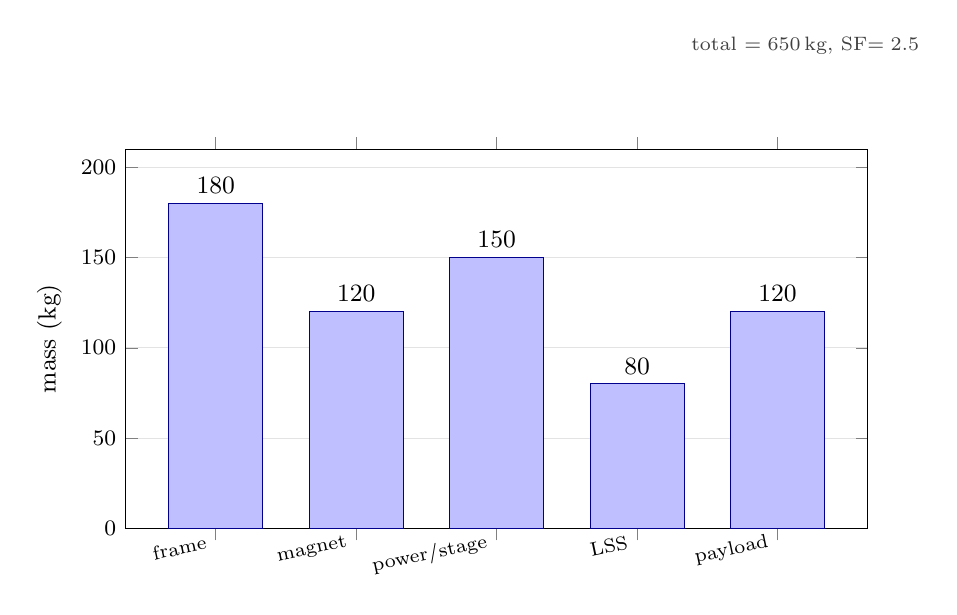
\begin{tikzpicture}
\begin{axis}[
  width=11cm, height=6.4cm,
  ybar,
  bar width=34pt,
  ymin=0, ymax=210,
  ylabel={mass (kg)},
  symbolic x coords={frame, magnet, {power/stage}, LSS, payload},
  xtick=data,
  x tick label style={font=\scriptsize, rotate=12, anchor=east},
  tick label style={font=\footnotesize},
  label style={font=\small},
  nodes near coords,
  nodes near coords style={font=\small},
  ymajorgrids, grid style={gray!22},
  enlarge x limits=0.16,
]
\addplot[draw=blue!55!black,fill=blue!25] coordinates {
  (frame,180) (magnet,120) ({power/stage},150) (LSS,80) (payload,120)
};
\end{axis}
\node[font=\scriptsize, gray!50!black, anchor=south east] at (10.2cm,5.9cm) {total $=650$\,kg, SF$=2.5$};
\end{tikzpicture}
\end{document}
